\title{Computational Neurophysiology - Exam 2}
\author{Ryan Spangler}
\date{\today}

\documentclass[12pt]{article}

\usepackage{commath}
\usepackage{graphicx}

\setcounter{secnumdepth}{0}

\begin{document}
\maketitle

\section{1. Spiking Neuron Models}

\subsection{A. Spike-Rate Adaptation}

Given an extra conductance in the integrate and fire model, more complex behavior can be attained, and some of the inherent limitations of the integrate and fire model can be mitigated.  One of the shortcomings of the integrate and fire model is the inability to adapt its firing rate.  Given a constant current, the integrate and fire model will fire at a constant rate, story over.  Adding another term corresponding to a activity-based damping current provides the necessary mechanism to model spike-rate adaptation.

Here is the form of the integrate and fire equation with the newly introduced adaptation term:

$$ \tau_m\od{V(t)}{t}=E_{leak}-V(t)-r_mg_{rsa}(V-E_k)+R_mI(t),\text{ where}$$

$$ \tau_{rsa}\od{g_{rsa}}{t}=-g_{rsa} $$

The conductance is modeled as a decaying exponential.  The other component to this is that whenever the model undergoes a spike, in addtion to setting $V=V_{spike}$, that 

$$ g_{rsa}=g_{rsa}+\Delta g_{rsa}$$

The model works if $\tau_{rsa}$ is slow enough to allow $g_{rsa}$ time to accumulate during periods of prolonged spiking.  If the input current quiets again the exponential decay will take over and reset $g_{rsa}$ back to zero.  

Here is the model in action, using $\Delta g_{rsa}=1$, $r_m=1$ and $tau_{rsa}=30$:

\vspace{15pt}
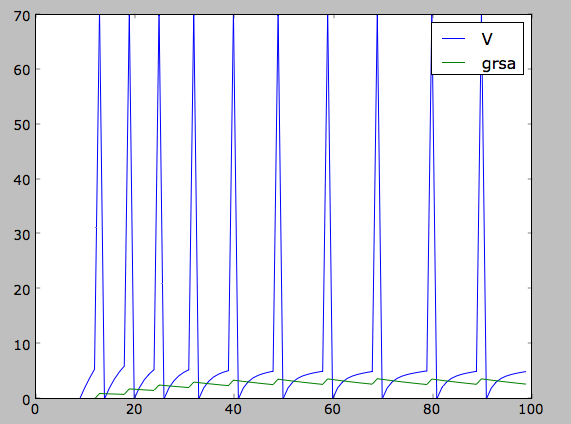
\includegraphics[scale=0.63]{adaptation.png}
\vspace{5pt}

The current is added at $t=10$ and sustained for the rest of the trial.  As is evident, the spike interval is initially short and lengthens as time goes on.  $g_{rsa}$ starts initially low, but during the period of high spiking rises more quickly than the decay governed by $\tau_{rsa}$.  Eventually the rate of firing balances the rate of decay, and $g_{rsa}$ hovers around a small range.  

This mechanism has the biological effect of adapting the firing rate to stimuli that do not change, and emphasizing {\em change} of stimuli rather than strength.  

\subsection{B. Refractory Periods}

Another shortcoming of the integrate and fire model is the inability to emulate a refractory period, one of the main features of neural spiking behavior.  The same kind of conductance as was used for spike rate adaptation could be used to model refractory periods as well.  A simple change to the values of the parameters is enough to model refractory periods: a rise in the height of $\Delta g_{rsa}$ and a lower $tau_{rsa}$ to make the decay more swiftly.  

Here is the behavior of the integrate and fire model with and without a refractory period, under a continuous stimulus amplitude of 5 nA:

\vspace{15pt}
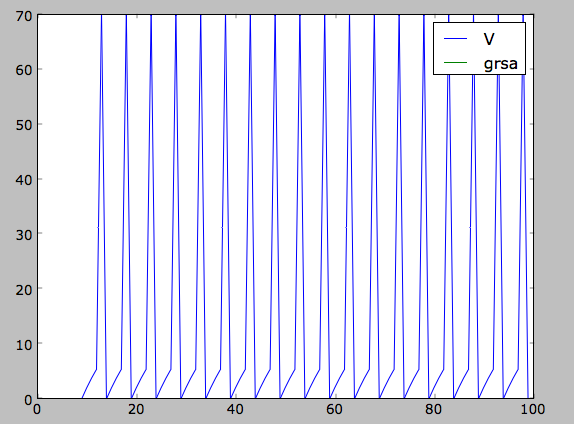
\includegraphics[scale=0.5]{vanillaif.png}
\vspace{5pt}

Here is the same neuron with a refractory period given by the same equations as the spike-rate adaptation current above, but this time with $\Delta g_{rsa}=20$ and $\tau_{rsa}=5$:

\vspace{15pt}
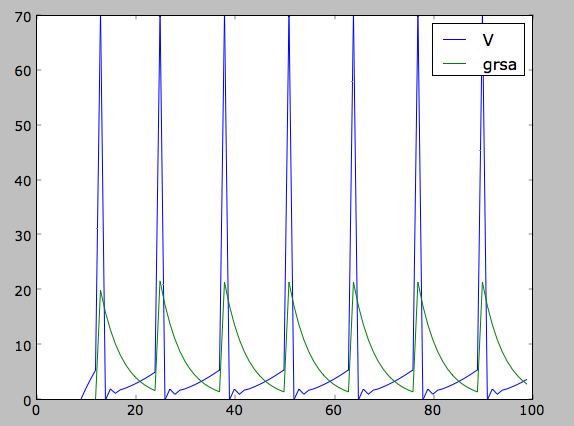
\includegraphics[scale=0.5]{refractory.png}
\vspace{5pt}

The behavior of the two models reveals that the refractory-period version is less responsive directly after a spike, while the original continues unfazed.  This results in a much more attenuated interspike interval in the model with the refractory current included, and thus a lower firing rate.

To model an absolute refractory period it would only be necessary to clamp $V=0$ for a given time span $t_{absolute}$.  This would not be any more contrived than the spike mechanism already is.  

\section{2. Population Decoding}

\subsection{A. Simulation}

The cercal system in the cricket is a population of four neurons whose relative firing rates encode wind direction.  Each is most responsive to a different orthogonal or opposite direction (a neuron is needed for each opposite direction because there is no encoding of a negative firing rate).  Together, these four neurons encode a cartesian plane.  

To encode the firing rates for a given angle the following formula is used:

$$ \langle r_i \rangle=[50cos(\theta-\theta_i)]_+ \text{ where}$$
$$ \theta_i=[\frac{\pi}{4},\frac{3\pi}{4},\frac{5\pi}{4},\frac{7\pi}{4}] $$

To obtain the firing rates we add a gaussian noise of 5hz to the these rates (to emulate the stochasticity of real neurons).  

To decode the wind direction from these relative firing rates, we can scale each neuron's preferred direction $\theta_i$ by its respective rate of firing $r_i$ to glean each components contribution to the overall encoding for wind direction.  

Plotting true wind direction to the estimated wind direction produces the following graph:

\vspace{15pt}
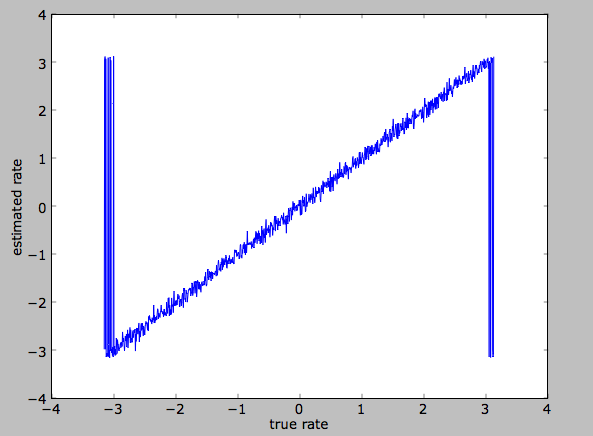
\includegraphics[scale=0.5]{truevsestimated.png}
\vspace{5pt}

The jumps at the end are because this is actually a cyclic number line, with $-\pi$ meeting up with $+\pi$ to form a continuous cycle.  The estimate is stochastic but follows pretty closely with the original angle.

For 1000 trials against each wind direction, the average error relative to each direction is

\vspace{15pt}
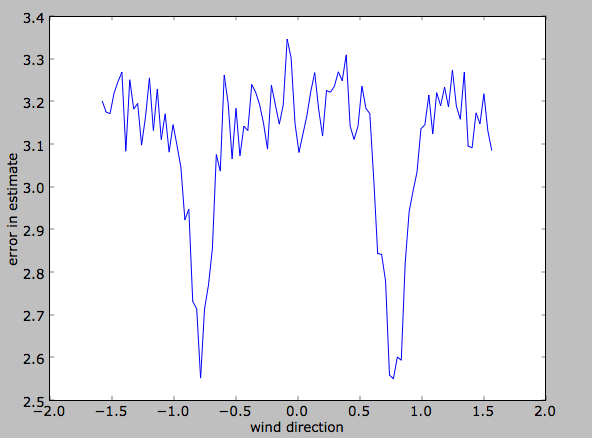
\includegraphics[scale=0.5]{estimationerror.png}
\vspace{5pt}

The large dips are around $-\frac{\pi}{4}$ and $\frac{\pi}{4}$, exactly where the neurons are most sensitive.  

\subsection{B. Discussion}

What is the source of the error?  Well, a large portion of it comes from the gaussian noise we added, the conditions are admittedly contrived.  But also, the dips in the second graph speak to another source of error, that of the ambiguity of the neuronal response when the stimulus lies between the sensitivites for each.  The response is least ambiguous when the stimulus is centered on one of the neuron's sensitivies, as this is the area where its response is strongest and the difference of firing between it and its neighbors is most marked.  When the stimulus is between sensitivies, both responses are noticeable yet equivalent, giving any noise inherent in the encoding process far more impact on the ultimate encoded direction.  

A number of things could be done to reduce the error.  First would be to add more neurons, subdividing the circle more times and providing a wider array of sensitivies to be accurate for.  This of course takes more space, and something maybe lost in clarity and applicability of representation what is added in granularity.  Another could be to reduce the field at which each neuron is responsive, or more closely fit the curve of sensitivity dropoff to what maximizes the difference between responses.  For areas between sensitivites this could enhance the distinction between neighboring neuron's firing strength.  Finally, adding two more neurons for the z-plane, or third dimension (up and down), could enhance the effective responsiveness in all directions.   .

\section{3. Phase Plane Analysis}

\subsection{A. Equilibrium}

The particular incarnation of the Fitzhugh-Nagumo model of the action potential for this problem is of the form

$$ \od{V}{t}=\frac{1}{\tau}(V-\frac{V^3}{3}-R+I_{input}) $$
$$ \od{R}{t}=\frac{1}{\tau_R}(1.25V-R+1.5) $$

where $\tau=0.1$ and $\tau_R=0.5$ (not 1.25 as is written.  0.5 is the value in the matlab simulation given and it is the one that has a distinction between I=1.0 and I=1.1).  

To determine the equilibrium points for a given stimulus amplitude we can find the roots of the equations that result from setting $\od{V}{t}=0$ and $\od{R}{t}=0$.  This amounts to solving the equation (after substituting R)

$$ \frac{V^3}{3}+.25V+1.5+I $$

For $I=0$ this turns out to be $[V,R]=[-1.5,-.375]$, $I=1.0$ gives $[V,R]=[-9.29,.338]$ and $I=1.1$ produces $[V,R]=[-.832,.459]$.  

In order to discover the behavior around the equilibrium points we must find the eigenvalues of the system at those points.  Deriving the Jacobian matrix from the original model and subtracting the as yet unknown eigenvalues multiplied by the identity $A-\lambda I$ from it gives a characteristic equation of 

$$ \lambda^2+(10V^2-8)\lambda+20V^2=0 $$

Finding the roots of this equation gives the eigenvalues of the various stimulus amplitudes as

$$ \lambda_{I=0}=-10,-4.5 $$
$$ \lambda_{I=1.0}=-.32+4.14\imath,-.32-4.14\imath $$
$$ \lambda_{I=1.1}=.54+3.68\imath,.54-3.68\imath $$

For $I=0$, the eigenvalues are both negative, meaning the equilibrium is a stable node.  When $I=1.0$ the eigenvalues are a complex conjugate pair with negative real parts, meaning the dynamics will spiral asymptotically towards the equilibrium point.  When $I=1.1$ the eigenvalues are also a complex conjugate pair, but this time the real part is positive, which means the behavior will spiral outwards from this point, and that it is ultimately unstable.  This does not mean however that there is not a limit cycle the equilibrium spirals towards asymptotically, which as it turns out is exactly what is happening.  For $I=1.0$ the model spikes once before settling into equilibrium.  For $I=1.1$, the system spikes recurrently about a limit cycle.

\subsection{B. Simulation}

The simulation of the Fitzhugh-Nagumo model reveals the validity of these conclusions.  When $I=1.0$, the variables spiral towards equilibrium.  When $I=1.1$, the spiral towards a limit cycle of spiking, no matter where they are in the phase plane.  This could be seen as due to the interaction between the linear R-nullcline and the cubic V-nullcline.  Increasing I raises the V-nullcline with respect to the R-nullcline, which remains constant, as can be seen in the next diagram:

\vspace{15pt}
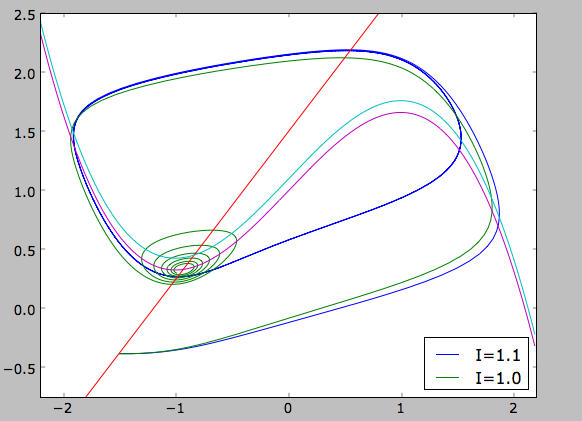
\includegraphics[scale=0.71]{phaseplane.png}
\vspace{5pt}

In this diagram, V (horizontal) is graphed relative to R (vertical).  The R-nullcline is red and the V-nullcline is cyan when $I=1.1$ and pink when $I=1.0$.  The intersection between the nullclines are the equilibrium points.  The green line is spiraling towards the intersection between the R-nullcline and the pink V-nullcline.  The intersection of the R-nullcline and the cyan V-nullcline provides a center to the action potential limit cycle.  The points at which the trajectories cross the nullclines the motion of that variable in that direction reverses.  To the right of the R-nullcline R is rising, but to the left it is falling.  Likewise, below the V-nullcline V is rising, but above it is falling.  This is where the oscillatory dynamics come from.  

So essentially, raising the stimulus current raises the V-nullcline, which means that more of the time the trajectory spends rising in V.  Since V is the activity, at a certain point (when the eigenvalues at the equilibrium point change from being negative real numbers to complex conjugate pairs) this translates from stable equilibrium points into single spikes.  This occurs for this system at $I=0.7$, a kind of tipping point into spiking behavior.  This threshhold is illustrated in the next diagram:

\vspace{15pt}
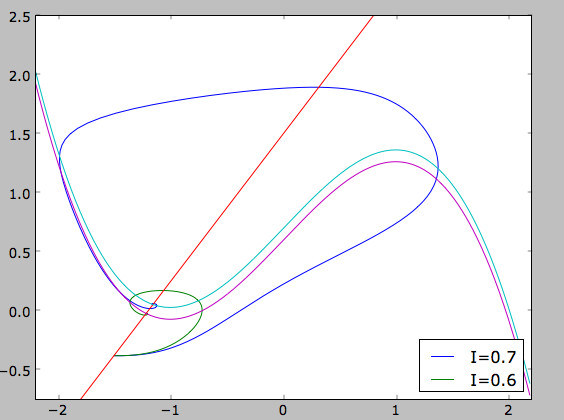
\includegraphics[scale=0.71]{phaseplanethreshhold.png}
\vspace{5pt}

In the non-spiking trajectory colored green, it does not gain enough V to escape the curl of the pink V-nullclines valley, and is quickly reabsorbed into the rest equilibrium.  The blue trajectory on the other hand corresponds to the higher cyan V-nullcline.  This trajectory clears the valley of the nullcline and travels all the way to the other side of the hill before crossing.  This is interpreted as a spike.  

Another phase shift occurs when the real part of the eigenvalues become positive, creating a limit cycle which translates into recurrent spiking.  

\section{4. Course Review}

\subsection{A. Calcium Channels}

L-type high-threshhold calcium channels function as activity monitors.  Since they only open at high potentials and deactivate in the presence of calcium, they raise the level of calcium to a particular saturation point when activity is high.  Since calcium is always being removed from the cytoplasm, calcium levels can only get to a certain point under the influence of heavy firing.  This makes calcium useful as a barometer of the general activity level of the cell at that point in time.  T-type low-threshhold calcium channels act as a slow sodium current, depolarizing enough to allow bursts of spikes before being counteracted by some other current, possibly a calcium-dependent potassium current.  L-type channels are closer to the soma so that they can have a more general effect on the activity of the neuron, whereas L-type channels are more distal in order to offer fine-grained impact onto the dynamics of each synapse.  

\subsection{B. Phase Locking}

When given two mutually inhibitory neurons, an oscillation or phase locking is almost inevitable.  To see this, imagine that both are innervated, one slightly before the other (this is realistic because no two signals are ever {\em exactly} simultaneous).  The one that is ahead of the game will inhibit the other before it has time to reciprocate.  The second will therefore fall silent as it labors under the inhibitory influence of the first.  When the activity of the first neuron inevitably falls, the second has been primed by hyperpolarization and rises to inhibit the first, which then falls silent.  The roles have reversed directly, and it is easy to see how this mutual back and forth interaction will perpetuate indefinitely, giving rise to oscillatory dynamics.

\subsection{C. Inhibition}

When an inhibitory synapse has a reversal potential very close to the resting potential of a cell, it can have a variety of effects.  Any activity poised to spike will be reduced towards rest, but if the cell is already hyperpolarized it could even have an excitatory effect.  Its main function is to neutralize the action of other excitatory or inhibitory connections, and has its greatest impact when located near the soma or proximal dentritic tree. 

\subsection{D. Stochastic Firing}

There are many possible explanations for the perceived stochasticity in the firing patterns of neurons.  The simplest, and most friendly, is that neurons work in rates and not individual spikes because the environment is inherently noisy, and the stochastic probability-correlation nature of the firing patterns allows a level of robustness in the face of environmental and internal noise.  The Poisson process of generating simulated spike trains is the canonical idealization of this explanation.  In it, the timing of each spike has no relation to the timing of any other spike.  If you squint, it almost looks like neurons follow this rule.  At least, no other obvious pattern is discernible most of the time, so the Poisson process is a pretty reasonable estimate in those cases.  

The other, more ominous explanation is that they appear to spike at random intervals because we don't actually understand why they are firing then.  Lacking an accurate explanation of the perceived spike timing of neurons, randomness is the comforting alternative.  The interval between spikes is dependent on so many factors across so many time scales and involving so many other spikes generated from other neurons that teasing apart all of the relations into a comprehensible explanation is almost intractable.  At least at the moment.  Poisson at its heart fails to account for this myriad network of relationships inherent in neuronal structure (or even the mutual information between spike times), and therefore will never actually describe network dynamics in an explanatory way.  

\end{document} 
